\documentclass[tikz,border=5pt]{standalone}
\usetikzlibrary{arrows.meta,decorations.pathreplacing,angles,quotes}
\usepackage{newtxmath}
\begin{document}
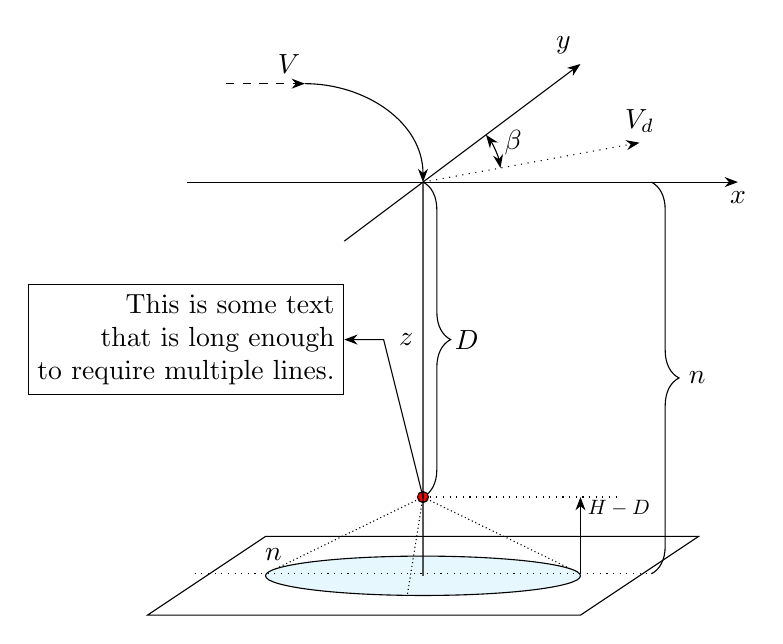
\begin{tikzpicture}[>=Stealth]
  \draw[->] (-3,0) -- (4,0) node[below] {$x$};
  \draw[->] (-1,-.75) -- (2,1.5) coordinate (y) node[above left] {$y$};
  \draw[->,dashed] (-2.5,1.25) -- node[pos=.8,above] {$V$} ++(1,0) coordinate (v);
  \draw[->,dotted] (0,0) coordinate (O) -- ++(2.75,0.5) coordinate (vd)  node[above] {$V_d$};
  \draw[->] (v) to[out=0,in=90] (O);
  \draw[fill=cyan!10] (0,-5) coordinate (center) ellipse[x radius=2, y radius=.25]; 
  \draw[decorate,decoration={brace,amplitude=10}] (0,0) -- node[right=8pt] {$D$} (0,-4);
  \draw[fill=red] (0,0) -- node[left] {$z$} (0,-4) coordinate (red) circle[radius=2pt] -- ++(0,-1);
  \pic["$\beta$",<->,draw,angle radius=1cm,angle eccentricity=1.25] {angle = vd--O--y};
  \draw[densely dotted] 
    (red) -- ++(1.9,-.925) coordinate (R)
    (red) -- ++(-1.9,-.925) coordinate (L) node[above] {$n$}
    (red) --++(-.2,-1.25);
    \draw[dotted] ([xshift=-1cm,yshift=-.05cm]L) -- ([xshift=+1cm,yshift=-.05cm]R) coordinate (h) (red) -- ++(2.5,0);
    \coordinate (aux) at ([xshift=.1cm,yshift=-.05cm]R);
    \draw[->] (aux) -- (aux|-red) node[pos=.85,right,scale=.75] {$H-D$};
    \draw[decorate,decoration={brace,mirror,amplitude=10}] (h) -- node[right=10pt] {$n$} (h|-O);
    \draw ([xshift=-3.5cm,yshift=-.5cm]center) -- ([xshift=+2cm,yshift=-.5cm]center) -- ([xshift=+3.5cm,yshift=.5cm]center) -- ([xshift=-2cm,yshift=.5cm]center) -- cycle;
    \draw[->] (red) -- ++(-.5,2) -- ++(-.5,0) node[draw,anchor=east,align=right] {This is some text\\that is long enough\\to require multiple lines.};
\end{tikzpicture}
\end{document}